%%%%%%%%%%%%%%%%%%%%%%%%%%%%%%%%%%%%%%%%%
% Beamer Presentation
% LaTeX Template
% Version 1.0 (10/11/12)
%
% This template has been downloaded from:
% http://www.LaTeXTemplates.com
%
% License:
% CC BY-NC-SA 3.0 (http://creativecommons.org/licenses/by-nc-sa/3.0/)
%
%%%%%%%%%%%%%%%%%%%%%%%%%%%%%%%%%%%%%%%%%

%----------------------------------------------------------------------------------------
%	PACKAGES AND THEMES
%----------------------------------------------------------------------------------------

\documentclass[UTF8,aspectratio=169,14pt]{ctexbeamer}

\usepackage{hyperref}
\hypersetup{
	colorlinks=true,
	linkcolor=red,
	anchorcolor=blue,
	citecolor=green
}

\mode<presentation> {
	
	% The Beamer class comes with a number of default slide themes
	% which change the colors and layouts of slides. Below this is a list
	% of all the themes, uncomment each in turn to see what they look like.
	
	%\usetheme{default}
	%\usetheme{AnnArbor}
	%\usetheme{Antibes}
	%\usetheme{Bergen}
	%\usetheme{Berkeley}
	%\usetheme{Berlin}
	%\usetheme{Boadilla}
	%\usetheme{CambridgeUS}
	%\usetheme{Copenhagen}
	%\usetheme{Darmstadt}
	%\usetheme{Dresden}
	%\usetheme{Frankfurt}
	%\usetheme{Goettingen}
	%\usetheme{Hannover}
	%\usetheme{Ilmenau}
	%\usetheme{JuanLesPins}
	%\usetheme{Luebeck}
	\usetheme{Madrid}
	%\usetheme{Malmoe}
	%\usetheme{Marburg}
	%\usetheme{Montpellier}
	%\usetheme{PaloAlto}
	%\usetheme{Pittsburgh}
	%\usetheme{Rochester}
	%\usetheme{Singapore}
	%\usetheme{Szeged}
	%\usetheme{Warsaw}
	
	% As well as themes, the Beamer class has a number of color themes
	% for any slide theme. Uncomment each of these in turn to see how it
	% changes the colors of your current slide theme.
	
	%\usecolortheme{albatross}
	%\usecolortheme{beaver}
	%\usecolortheme{beetle}
	%\usecolortheme{crane}
	%\usecolortheme{dolphin}
	%\usecolortheme{dove}
	%\usecolortheme{fly}
	%\usecolortheme{lily}
	%\usecolortheme{orchid}
	%\usecolortheme{rose}
	%\usecolortheme{seagull}
	%\usecolortheme{seahorse}
	%\usecolortheme{whale}
	%\usecolortheme{wolverine}
	
	%\setbeamertemplate{footline} % To remove the footer line in all slides uncomment this line
	%\setbeamertemplate{footline}[page number] % To replace the footer line in all slides with a simple slide count uncomment this line
	
	%\setbeamertemplate{navigation symbols}{} % To remove the navigation symbols from the bottom of all slides uncomment this line
}

\usepackage{graphicx} % Allows including images
\graphicspath{{./figs/}}
\usepackage{booktabs} % Allows the use of \toprule, \midrule and \bottomrule in tables
\usepackage{longtable}
\usepackage{listings}
\usepackage{xcolor}
\lstset{numbers=left, %设置行号位置
	numberstyle=\tiny, %设置行号大小
	keywordstyle=\color{blue}, %设置关键字颜色
	commentstyle=\color[cmyk]{1,0,1,0}, %设置注释颜色
	frame=single, %设置边框格式
	escapeinside=``, %逃逸字符(1左面的键),用于显示中文
	%breaklines, %自动折行
	extendedchars=false, %解决代码跨页时,章节标题,页眉等汉字不显示的问题
	xleftmargin=2em,xrightmargin=2em, aboveskip=1em, %设置边距
	tabsize=4, %设置tab空格数
	showspaces=false %不显示空格
}
% Fonts
% \usepackage{libertine}
% \setmonofont{Courier}
\setCJKsansfont[ItalicFont=Noto Serif CJK SC Black, BoldFont=Noto Sans CJK SC Black]{Noto Sans CJK SC}


%----------------------------------------------------------------------------------------
% TITLE PAGE
%----------------------------------------------------------------------------------------

\title[第19讲]{第十九讲 :I/O子系统} % The short title appears at the bottom of every slide, the full title is only on the title page
\subtitle{第5节:Linux I/O子系统}
\author{向勇、陈渝、李国良} % Your name
\institute[清华大学] % Your institution as it will appear on the bottom of every slide, may be shorthand to save space
{
  清华大学计算机系 \\ % Your institution for the title page
  \medskip
  \textit{xyong,yuchen,liguoliang@tsinghua.edu.cn} % Your email address
}
\date{\today} % Date, can be changed to a custom date

\begin{document}

\begin{frame}
\titlepage % Print the title page as the first slide
\end{frame}

%----------------------------------------------
\begin{frame}
\frametitle{提纲} % Table of contents slide, comment this block out to remove it
\tableofcontents % Throughout your presentation, if you choose to use \section{} and \subsection{} commands, these will automatically be printed on this slide as an overview of your presentation

%% itemize
Ref:
    \begin{itemize}
        \item \href{http://osq.cs.berkeley.edu/public/JFoster-Drivers.ppt}{Linux Device Drivers Overview}
        \item \href{http://ermak.cs.nstu.ru/understanding.linux.kernel.pdf}{Understanding the Linux Kernel}
    \end{itemize}

\end{frame}
%----------------------------------------------
%%  PRESENTATION SLIDES
%----------------------------------------------
\section{第5节:Linux I/O子系统} % Sections can be created in order to organize your presentation into discrete blocks, all sections and subsections are automatically printed in the table of contents as an overview of the talk
%----------------------------------------------
\subsection{Linux I/O Architecture} % A subsection can be created just before a set of slides with a common theme to further break down your presentation into chunks
%----------------------------------------------
\begin{frame}[fragile]
    \frametitle{Linux I/O Architecture}
%    \framesubtitle{xxxx}
%% figure
    \begin{figure}
    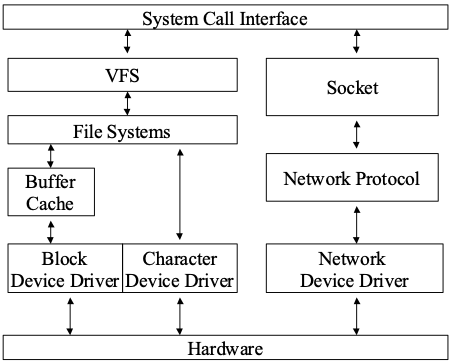
\includegraphics[width=0.57\linewidth]{figs/io-architecture.png}
  %  \caption{xxxx}
    \end{figure}
\end{frame}
%----------------------------------------------
% #### Linux I/O Architecture
% 
% ##### Linux I/O Architecture
% 
% ![io-architecture](figs/io-architecture.png)
% 
%----------------------------------------------
\begin{frame}[fragile]
    \frametitle{Block Driver}
%    \framesubtitle{xxxx}
%% figure
    \begin{figure}
    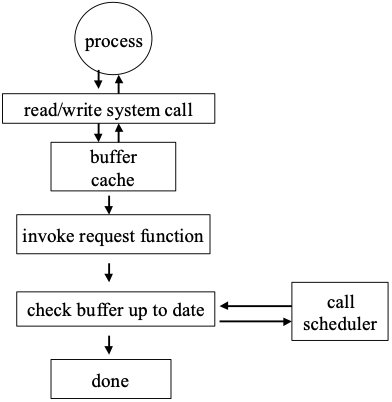
\includegraphics[width=0.47\linewidth]{figs/block-driver.png}
  %  \caption{xxxx}
    \end{figure}
\end{frame}
%----------------------------------------------
% ##### Block Driver
% 
% ![block-driver](figs/block-driver.png)
% 
%----------------------------------------------
\begin{frame}[fragile]
    \frametitle{Network Driver}
%    \framesubtitle{xxxx}
%% figure
    \begin{figure}
    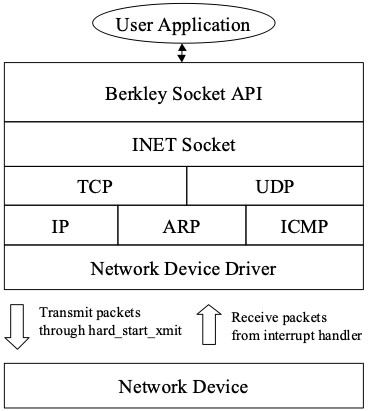
\includegraphics[width=0.42\linewidth]{figs/network-driver.png}
  %  \caption{xxxx}
    \end{figure}
\end{frame}
%----------------------------------------------
% ##### Network Driver
% 
% ![network-driver](figs/network-driver.png)
% 
%----------------------------------------------
\subsection{Device Driver} % A subsection can be created just before a set of slides with a common theme to further break down your presentation into chunks
%----------------------------------------------
\begin{frame}[fragile]
    \frametitle{Device Driver interface}
%    \framesubtitle{xxxx}
%% figure
    \begin{figure}
    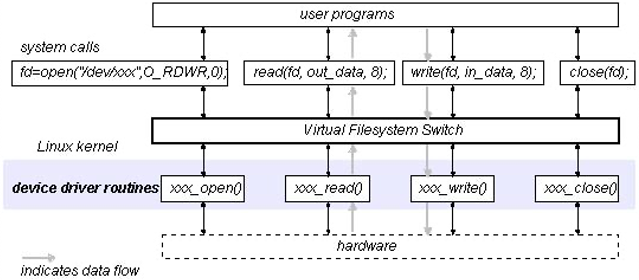
\includegraphics[width=0.9\linewidth]{figs/driver-interface.png}
  %  \caption{xxxx}
    \end{figure}
\end{frame}
%----------------------------------------------
% #### Device Driver
% 
% ##### Device Driver interface
% 
% ![driver-interface](figs/driver-interface.png)
% 
%----------------------------------------------
\begin{frame}[fragile]
    \frametitle{Interface between a Device Driver and Linux Kernel}
%    \framesubtitle{xxxx}
%% figure
    \begin{figure}
    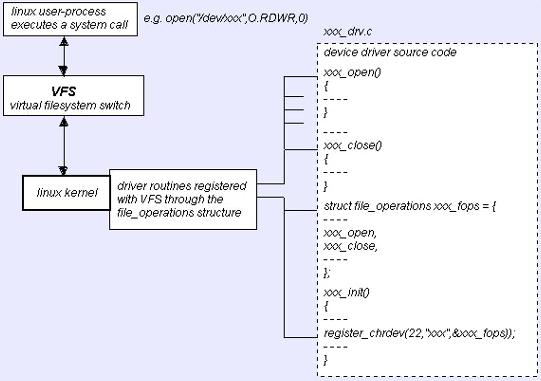
\includegraphics[width=0.65\linewidth]{figs/kernel-interface.png}
  %  \caption{xxxx}
    \end{figure}
\end{frame}
%----------------------------------------------
% ##### Interface between a Device Driver and Linux Kernel
% 
% ![kernel-interface](figs/kernel-interface.png)
% 
%----------------------------------------------
\begin{frame}[fragile]
    \frametitle{Device Driver Implementation}
%    \framesubtitle{xxxx}
Assuming that your device name is xxxx
    \begin{itemize}
        \item xxxx\_init() initialize the device when OS is booted
        \item init\_module()
        \item cleanup\_module() \pause
        \item xxxx\_open() open a device 
        \item xxxx\_read() read from kernel memory 
        \item xxxx\_write() write 
        \item xxxx\_release() clean-up (close)
    \end{itemize}
\end{frame}
%----------------------------------------------
% ##### Device Driver Implementation
% 
% Assuming that your device name is xxxx
%  * xxxx_init() initialize the device when OS is booted
%  * xxxx_open() open a device 
%  * xxxx_read() read from kernel memory 
%  * xxxx_write() write 
%  * xxxx_release() clean-up (close)
%  * init_module()
%  * cleanup_module()
% 
%----------------------------------------------
\begin{frame}[fragile]
    \frametitle{Kernel Support Functions}
%    \framesubtitle{xxxx}
    \begin{itemize}
        \item I/O ports reservations
        \begin{itemize}
            \item request\_region()
        \end{itemize}
        \item Interrupt Handler Registration
        \begin{itemize}
            \item request\_irq()
        \end{itemize} \pause
        \item Memory Allocations   
        \begin{itemize}
            \item kmalloc(), vmalloc(), get\_free\_page()
        \end{itemize} \pause
        \item Data Transfer between User/Kernel
        \begin{itemize}
            \item memcpy\_fromfs()
        \end{itemize}
    \end{itemize}
\end{frame}
%----------------------------------------------
% ##### Kernel Support Functions
% 
%  * I/O ports reservations
%     * request_region()
%  * Memory Allocations   
%     * kmalloc(), vmalloc(), get_free_page()
%  * Interrupt Handler Registration
%     * request_irq()
%  * Data Transfer between User/Kernel
%     * memcpy_fromfs()
% 
%----------------------------------------------
\subsection{Device Driver Programming} % A subsection can be created just before a set of slides with a common theme to further break down your presentation into chunks
%----------------------------------------------
\begin{frame}[fragile]
    \frametitle{API requirements}
%    \framesubtitle{xxxx}
    \begin{itemize}
        \item Driver functions return positive ints on success, negative ints on failure
        \item Kernel won’t call non-blocking I/O functions if previous request still pending
        \item Every kernel function that calls kmalloc() should be reentrant \pause
        \item Common Mistakes
        \begin{itemize}
            \item Locking, Interrupt time, resource allocation
        \end{itemize}
    \end{itemize}
\end{frame}
%----------------------------------------------
% #### Device Driver Programming
% 
% ##### API requirements
% 
% ref: JFoster-Drivers.ppt - Page 4
% 
%  * Driver functions return positive ints on success, negative ints on failure
%  * Kernel won’t call non-blocking I/O functions if previous request still pending
%  * Every kernel function that calls kmalloc (GFP_KERNEL) should be reentrant
%  * Common Mistakes
%     * Locking, Interrupt time, resource allocation
% 
%----------------------------------------------
\begin{frame}[fragile]
    \frametitle{Locking}
%    \framesubtitle{xxxx}
    \begin{itemize}
        \item Four kinds of locks in kernel
        \begin{itemize}
            \item Spin locks and read-write locks
            \item Interrupt enable/disable
            \begin{itemize}
                \item Sometimes combined, e.g., spin\_lock\_irq
            \end{itemize}
            \item Whole kernel lock
        \end{itemize} \pause
        \item Locks are used all over the place
        \begin{itemize}
            \item Are they used correctly?  consistently?
        \end{itemize}
    \end{itemize}
\end{frame}
%----------------------------------------------
% ##### Locking
%  * Four kinds of locks in kernel
%     * Spin locks and read-write locks
%     * Interrupt enable/disable
%        * Sometimes combined, e.g., spin_lock_irq
%     * Whole kernel lock
%  * Locks are used all over the place
%     * Are they used correctly?  consistently?
% 
%----------------------------------------------
\begin{frame}[fragile]
    \frametitle{Interrupt Time}
%    \framesubtitle{xxxx}
When in\_interrupt is true, code cannot \pause
    \begin{itemize}
        \item Access current
        \item Call the scheduler (may sleep)
        \item Call kmalloc() (may sleep)
        \item Copy to/from user-space (may sleep)
        \item more?
    \end{itemize}
\end{frame}
%----------------------------------------------
% ##### Interrupt Time
% 
% When in_interrupt is true, code cannot
%  * Access current
%  * Call the scheduler (may sleep)
%  * Call kmalloc(GFP_KERNEL) (may sleep)
%  * Copy to/from user-space (may sleep)
%  * more?
% 
%----------------------------------------------
\begin{frame}[fragile]
    \frametitle{Resource Allocation}
%    \framesubtitle{xxxx}
    \begin{itemize}
        \item Drivers get and release system resources
        \begin{itemize}
            \item Memory
            \item IRQs
            \item module numbers (maybe)
            \item space for their code (mod usage count)
        \end{itemize} \pause
        \item Are the resources handled correctly?
        \begin{itemize}
            \item Leaks lead to instability -- reboot to reclaim
        \end{itemize}
    \end{itemize}
\end{frame}
%----------------------------------------------
% ##### Resource Allocation
% 
%  * Drivers get and release system resources
%     * Memory
%     * IRQs
%     * module numbers (maybe)
%     * space for their code (mod usage count)
%  * Are the resources handled correctly?
%     * Leaks lead to instability -- reboot to reclaim
%----------------------------------------------
\end{document}
